\documentclass{article}
\usepackage{arxiv}

\usepackage[utf8]{inputenc}
\usepackage[english, russian]{babel}
\usepackage[T1]{fontenc}
\usepackage{url}
\usepackage{booktabs}
\usepackage{amsfonts}
\usepackage{nicefrac}
\usepackage{microtype}
\usepackage{lipsum}
\usepackage{graphicx}
\usepackage{natbib}
\usepackage{doi}

\def\vec#1{\mathchoice{\mbox{\boldmath$\displaystyle#1$}}
{\mbox{\boldmath$\textstyle#1$}} {\mbox{\boldmath$\scriptstyle#1$}} {\mbox{\boldmath$\scriptscriptstyle#1$}}}

\title{Методы пространственной интерполяции в задаче пространственной интерполяции для оценки характеристик лесного массива}

\author{Гуров С.И.\\
	МГУ им. М.В. Ломоносова\\
	факультет ВМК\\
        119991, Москва, Ленинские горы, д.1, стр. 52\\
	\texttt{sgur@cs.msu.ru} \\
	\And
	  Илларионова С.В.\\
	  Сколковский институт науки и технологий\\
	121205, г. Москва, тер. Сколково Инновационного Центра, б-р Большой, д.30 стр. 1\\
	\texttt{s.illarionova@skoltech.ru} \\
    \And
    Глазырина С.Е. \\
	МГУ им. М.В. Ломоносова\\
	факультет ВМК\\
        119991, Москва, Ленинские горы, д.1, стр. 52\\
	\texttt{sv.glazyr@gmail.com} \\
}
\date{}

\renewcommand{\shorttitle}{\textit{arXiv} Template}

%%% Add PDF metadata to help others organize their library
%%% Once the PDF is generated, you can check the metadata with
%%% $ pdfinfo template.pdf
\hypersetup{
pdftitle={My first paper Glazyrina},
pdfkeywords={timber stock estimation, kriging},
}

\begin{document}
\maketitle

\begin{abstract}
В сферах экологического мониторинга и лесоводства оценка характеристик лесного покрова является ключевым фактором принятия решений. Картирование этих характеристик только на основе полевых измерений затруднительно, поэтому в настоящее время актуально построение моделей, позволяющих на основе имеющихся данных таксации и дополнительных признаков, таких как снимки, полученные спутниками или беспилотниками, получать более точные оценки характеристик леса. В данной работе сравнивается несколько получивших наибольшее распространение в последние годы методов оценки запасов древесины: логические модели, методы геостатистики, подходы частичного обучения. Предложена модификация "Впишу как только придумаю". Предложенный метод не принёс значительного улучшения качества, но работа может быть актуальна как сравнительный анализ использованных методов.
\end{abstract}


\keywords{пространственная интерполяция \and оценка запасов древесины}

\section*{Введение}
Знание характеристик лесного покрова необходимо во многих областях, таких как экологический мониторинг и охрана природы, лесное хозяйство, территориальное планирование. Особенно эти данные важны для обеспечения устойчивого лесопользования.

Запас древесины - один из ключевых факторов в управлении лесным хозяйством. Обычно он оценивается в ходе полевых измерений. Однако, из-за высокой стоимости и низкой доступности удалённых от дорог и рек лесных участков, количество проводимых во время таксации леса измерений остаётся ограниченным, а измерения - разреженными. Наша задача состоит в картировании запасов древесины местности на основе этих немногих измерений. Для решения проблемы недостатка данных многие исследователи, не только в задачах лесоводства, но и других задачах оценки окружающей среды, прибегают к дистанционному зондированию Земли. Использование таких признаков позволяет заметно повысить качество оценки.

\subsection*{Обзор литературы}

В последние годы с ростом доступности дистанционного зондирования для оценки запасов древесины помимо данных лесного кадастра, имеющихся лишь для малого числа точек области из-за высоких трудозатрат, связанных с их получением, в качестве дополнительных данных стали использоваться спутниковые снимки и данные, полученные с помощью лидара \citep{maack2016modelling}. Как показывает практика, использование этих данных, даже без учёта пространственных переменных, уже позволяет добиться хорошей точности в задаче оценки объемов древесины. В статье \cite{sanchez2019growing} описан ряд признаков, получаемых на основе этих данных и дающих наибольший вклад в решение этой задачи.

При рассмотрении данной задачи естественным кажется предположение о пространственной непрерывности целевой переменной. Оно является базовым для всех методов пространственной интерполяции. Простейшие детерминистические методы пространственной интерполяции, широко использовавшиеся в 90-е годы, такие как метод радиальных базисных функций или полиномиальные интерполяторы, позволяют использовать информацию о координатах точки измерения для оценки целевой переменной в этой точке \citep{kanushin2023review}. Если усилить постановку задачи предположением о пространственной стационарности целевой переменной, то к рассмотрению доступных методов добавляется группа стохастических методов типа кригинга - в зависимости от предположений о поведении среднего значения переменной можно использовать как простой (среднее значение известно и постоянно), обыкновенный (среднее значение неизвестно и постоянно во всей области оценивания) или универсальный (среднее значение неизвестно и непрерывно изменяется в области оценивания) кригинг \citep{geostatics_book}. Их преимущество состоит в поиске не только оценки целевой величины, но и оценке дисперсии ошибки, но предположение о стационарности существенно \citep{krukova2018spatialinterpolation}. Предположения можно ослабить, используя метод для оценивания значений в некоторой ограниченной подобласти (например, учитывать лишь точки, находящиеся от точки, в которой производится оценивание, не далее заданного порога), а не как глобальный интерполятор. Но ни один из этих методов не способен учесть информацию о дополнительных признаках. Для решения этой проблемы можно применить кригинг с внешним дрейфом, который использует дополнительные данные измерений коррелированной переменной в качестве модели тренда, и потому позволяет достаточно точно оценить тренд при наличии данных дополнительной тренд-переменной во всех точках оценивания \citep{hudson1994mapping}. Другой способ учесть дополнительные признаки - использование кокригинга - обобщение кригинга на случай многих переменных, предполагающий, что между ними есть пространственная корреляция \cite{wackernagel1995multivariate}.

В последние годы для решения подобных задач чаще стали использоваться различные нейросетевые архитектуры. При анализе пространственно-временных зависимостей достаточно удачным оказался подход из комбинации LSTM и некоторого блока Geo-Layer (реализации которого различны в разных работах), позволяющего учесть пространственную корреляцию \citep{sanchez2019growing, MA2019117729, maack2016modelling}. Кроме этого, использованные в статье \cite{MA2019117729} методы машинного обучения, в частности случайный лес, показали лучший по сравнению с традиционными методами геостатистики и нейросетевыми архитектурами результат при рассмотрении пространственно скоррелированных данных. В статье \citep{LIU2011568} предлагается архитектура нейронной сети, использующая радиальные базисные функции. Для экспериментов, проведённых в этой статье, такая нейронная сеть оказалась лучшим пространственным интерполятором, по сравнению с кригингом, так как не требует выполнения множества предположений кригинга, но при этом получаемая функция координат не является непрерывной. В статье \cite{maack2016modelling} предлагается сравнение GAM и случайного леса на задаче оценки запасов древесины. Полученные ими результаты говорят о более высокой эффективности применения GAM для больших и разнородных участков, что не так интересно в нашем случае. При этом в ряде других исследований применение ансамбля из деревьев давало более высокий по сравнению с GAM результат.

Ведутся исследования в области разработки новых методов пространственной интерполяции. Зачастую они являются комбинацией известных детерминированных алгоритмов и методов машинного обучения. Например, в статье \cite{kataev2013classification} объекты обучающей выборки сначала разбиваются на кластеры со схожими свойствами, после чего интерполятор при оценке учитывает только объекты из того кластера, в котором находится точка оценивания.
Решаемую задачу можно переформулировать в терминах обучения с частичным привлечением учителя. Исследования в этой области ведутся уже достаточно давно, и существует целая иерархия методов регрессии в задаче частичного обучения \citep{Kostopoulos2018, Xu2021SSR}.


Задачей этого исследования является сравнение описанных выше подходов к пространственной интерполяции данных о запасе древесины. Кроме того, целью исследования является предложение собственной модификации "Вписать позже, в зависимости от того, что будет лучше работать" и оценки применимости предложенного метода.

\section{Используемые данные}

Вся эта работа возникла вокруг определённого набора данных, предложенного в статье \citep{Illarionova2024timberstock}. Кратко опишем его.
Набор представляет собой объединение 2 типов данных: данные лесного кадастра, полученные с помощью полевых измерений, и данные, полученные с помощью дистанционного зондирования.

\subsection{О данных лесного кадастра}

Данные были собраны на территории Колвинского лесничества, в северной части Пермского края, на границе с республикой Коми. Лесничество находится в зоне тайги на Среднем Урале. На основе возраста и разнообразия представленных видов деревьев, исследуемый регион можно разделить на 2 участка. Центральная и южная части лесничества представляют собой вторичный лес, сформировавшийся после массовой вырубки в 70-90х годах. Северная часть представлена же нетронутыми лесами, где влияние человека мало проявляется.
Каждый пробный участок представляет собой небольшой участок леса, на котором проводились полевые измерения. Пробные участки расположены в двухкилометровой зоне относительно рек и дорог. Каждый участок представляет собой круг радиусом 9 метров, все участки сгруппированы в кластеры. Каждый кластер состоит из 9 участков, расположенных в виде узлов решётки $3 \times 3$. Для каждого участка есть записи о представленных видах деревьев, их состоянии (живые или мёртвые), характеристиках развития стволов (изгиб, наличие верхушки, ветвление). Также представлены такие усреднённые характеристики, как высота деревьев, объём древесины (в м$^3$/га), диаметр ствола, возраст. Причём усреднённые данные имеются как по всему объему деревьев на участке, так и по отдельным видам. Всего имеется 693 измерения.

\subsection{О дополнительных данных}
Данный датасет включает мультиспектральные снимки со спутника Sentinel-2 L2A за 2022 и 2023 года, полученные из Google Earth Engine. Пространственное разрешение оригинальных снимков (в использумеых диапазонах) - от 10 до 20 метров на пиксель, но в ходе предобработки оно приведено к 10 метрам для всех исследуемых диапазонов частот, а пиксели получены как медианы по изображениям, где это пиксель не был облаками. Используются 10 каналов из 13 (B02-B8A, B11, and B12). Кроме этого, на основе спектральных данных рассчитаны вегетационные индексы (NDVI и EVI). 

На основе результатов лазерного сканирования, собранных в 2022 году, к данным добавлена модель высот крон. На основе спутниковых данных, сгенерирована цифровая модель рельефа (высоты над уровнем моря). Разрешение всех этих данных приведено к разрешению спутниковых снимков. Также добавлены данные о возрасте деревьев, полученные методами машинного обучения.

\begin{figure}[h]
    \centering
    \begin{tabular}{cc}
        \begin{subfigure}
            \centering
            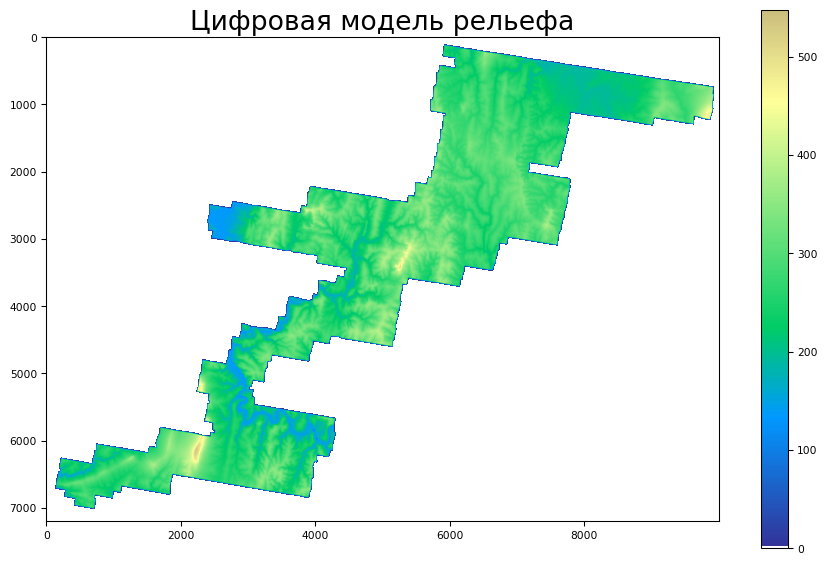
\includegraphics[width=0.48\textwidth]{images/DEM.png}
            \label{fig:dem}
        \end{subfigure}
        &
        \begin{subfigure}
            \centering
            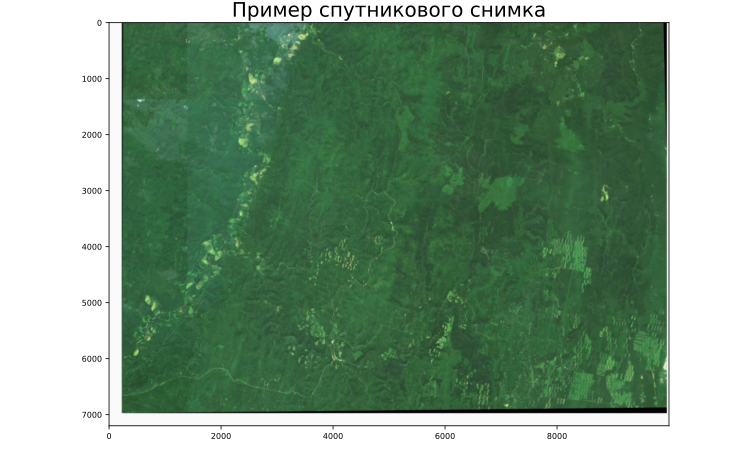
\includegraphics[width=0.48\textwidth]{images/satellite.pdf}
            \label{fig:sentinel}
        \end{subfigure}
        \\[1em]
        \begin{subfigure}
            \centering
            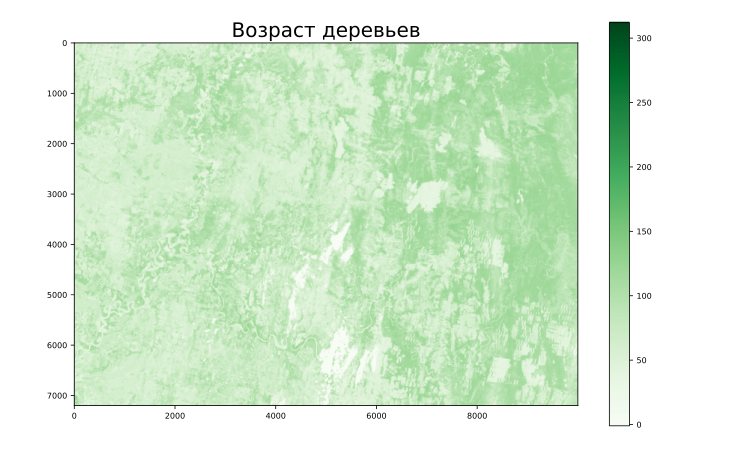
\includegraphics[width=0.48\textwidth]{images/age.pdf}
            \label{fig:age}
        \end{subfigure}
        &
        \begin{subfigure}
            \centering
            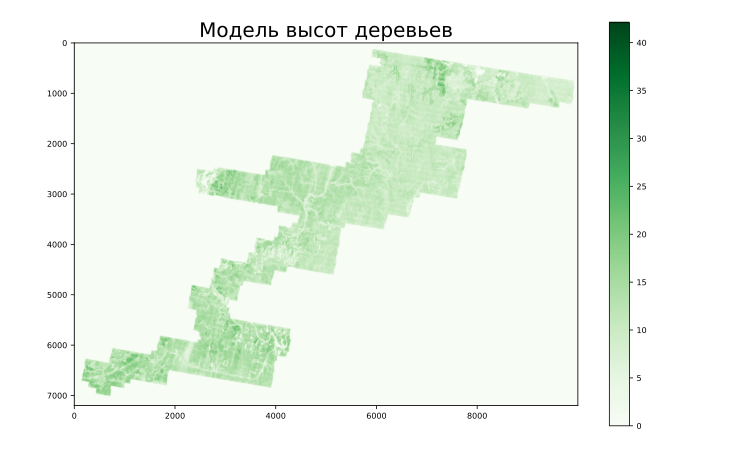
\includegraphics[width=0.48\textwidth]{images/chm.pdf}
            \label{fig:height}
        \end{subfigure}
    \end{tabular}
    \caption{Визуализация используемых данных}
    \label{fig:remote_sensing_data}
\end{figure}

\section{Постановка задачи}
Имеется два множества, $L = ((\vec{z}_1, t_1), ..., (\vec{z}_n, t_n))$, $x_i \in \mathbb{R}^{d}$, $t_i \in \mathbb{R}$ и $U = (\vec{z}_{n+1}, ..., \vec{z}_N)$, $u_i \in R^{d}$. все объекты $z_i, i=\overline{1, N}$ принадлежат одной генеральной совокупности. Необходимо построить модель, прогнозирующую $t$ для новых $x$. Такая постановка позволяет рассмотреть задачу частичного обучения для регрессии.

Теперь забудем о существовании неразмеченной части данных. Примем во внимание, что $\vec{z} \in \mathbb{R}$ также включает в себя значения координат объекта. Будем считать, что $t = t(x, y) + $. 



\section{Базовый эксперимент}
В рамках базового эксперимента применены следующие модели и методы: случайный лес, обычный кригинг, метод обратно-взвешенных расстояний, Semi-Supervised Kernel Regression.
\subsection{Описание методов}

Случайный лес - это ансамблевый метод машинного обучения, основанный на построении множества решающих деревьев, относящихся к семейству логических моделей, и последующем усреднении их прогнозов. Каждое дерево в лесу обучается независимо с использованием двух ключевых принципов рандомизации:
\begin{itemize}
    \item Бутстрэп (Bootstrap) - для каждого дерева создается своя обучающая выборка путем случайного выбора с возвращением $n$ объектов из исходной выборки размера $n$.
    \item Случайное подпространство признаков (Random Subspace) - при построении каждого узла дерева рассматривается только случайное подмножество признаков размера $m$ (обычно $m = d / 3$ для задач регрессии).
\end{itemize}


Обычный кригинг  - это метод пространственной интерполяции (то есть целевая функция представляется случайной функцией координат), основанный на предположении, что среднее значение процесса является неизвестной константой. Как и все методы кригинга, он даёт лучшую (с точки зрения минимизации дисперсии) несмещённую оценку и позволяет найти доверительные интервалы для этой оценки (из несмещённости следует, что метод является точным интерполятором, что не всегда удобно). Обычный кригинг не подразумевает использование дополнительных признаков.
Математическая формулировка: Пусть $T(s)$ - пространственный процесс, где $s$ - координаты точки. В обычном кригинге предполагается: $T(s) = \mu + \delta(s)$, где $\mu$ - неизвестное среднее (константа), $\delta(s)$ - стационарный случайный процесс с нулевым средним. Оценка в точке $s_0$ ищется как линейная комбинация наблюдений:
$$\hat{Z}(s_0) = \sum_{i=1}^n \lambda_i Z(s_i)$$
Веса $\lambda_i$ находятся из системы уравнений:
$$\begin{cases}
\sum\limits_{j=1}^n \lambda_j \gamma(s_i - s_j) + \mu = \gamma(s_i - s_0), \quad i = 1,\ldots,n \
\sum\limits_{i=1}^n \lambda_i = 1
\end{cases}$$
где: $\gamma(h)$ - вариограмма, $\mu$ - множитель Лагранжа. Условие $\sum \lambda_i = 1$ обеспечивает несмещённость оценки.

Метод обратно-взвешенных расстояний (Inverse Distance Weighting, IDW) является одним из базовых детерминистических методов геостатистики. В терминах машинного обучения, его можно назвать частным случаем ядерного сглаживания. Данный метод пространственной интерполяции основан на предположении, что объекты, расположенные ближе друг к другу, более похожи, чем удаленные объекты.
Математическая формулировка:
$$\hat{t}(s_0) = \frac{\sum_{i=1}^n w_i t(s_i)}{\sum_{i=1}^n w_i}$$
где: $\hat{t}(s_0)$ - оцениваемое значение в точке $s_0$, $z(s_i)$ - известные значения в точках измерений, $w_i$ - веса, обычно определяемые как: $w_i = \frac{1}{\rho(s_0, s_i)^p}$, $\rho(s_0, s_i)$ - расстояние между точкой интерполяции и точкой измерения, а $p$ - степенной параметр (обычно = 2), контролирующий скорость убывания весов с расстоянием. 

Semi-Supervised Kernel Regression (SSKR) - это метод, комбинирующий преимущества ядерной регрессии с возможностью использования как размеченных, так и неразмеченных данных. Использования ядерных фуннкций для нелинейного отображения данных и учёт структуры неразмеченных данных представляют особый интерес в исследуемой задаче.
Математическая формулировка:
$$\hat{t}(x) = \arg\min_{f \in \mathcal{H}} \left( \sum_{i=1}^n (y_i - f(x_i))^2 + \lambda_1 \sum_{i=n+1}^{N} (f(x_i) - \hat{y}_i)^2 + \lambda_2 \dot |f|^2_{\mathcal{H}} \right)$$
где: $n$ - количество размеченных примеров, $N$ - общее количество примеров, $\lambda_1, \lambda_2$ - параметры регуляризации, $\mathcal{H}$ - пространство функций с воспроизводящим ядром,
$\hat{y}_i$ - псевдометки для неразмеченных данных


\subsection{Ход эксперимента}
Описать подбор гиперпараметров для случайного леса (максимальная глубина и количество деревьев в ансамбле), вариациограмму для кригинга (здесь также будет график эмпирической вариограммы) (в качестве функции внешнего дрейфа предполагается использование результата некоторой регрессии от всех остальных признаков (с той же целевой переменной. Получаю что-то типа бустинга (правда лишь из 2 этапов... Но идея та же, если буду обучать кригинг на ошибки регрессиии... Или лучше даже наоборот - регрессию на ошибку кригинга - вот и не базовый эксперимент)? - по сути это уже собственная модификация известного метода)), ядро для SSKR.

\subsection{Метрики качества}
Для оценки полученных моделей, использованы следующие метрики: Mean Absolute Error ($MAE$), Root Mean Squared Error ($RMSE$), Mean Absolute Percentage Error ($MAPE$).

Пусть $t_i$ - наблюдаемое значение целевой переменной для объекта $x_i$, $\hat{t}_i$ - предсказанное значение для $x_i$, $n$ - число объектов в выборке.

$$MAE = \frac{1}{n}\sum_{i = 1}^n|t_i - \hat{t}_i|$$
MAE измеряет среднюю абсолютную разницу между предсказанными и фактическими значениями в единицах целевой переменной. Являясь линейной метрикой, MAE одинаково взвешивает все ошибки независимо от их величины, что делает её устойчивой к выбросам и особенно полезной при наличии шума в данных.

$$RMSE  = \sqrt{\frac{1}{N}\sum_{i=1}^n(t_i - \hat{t}_i)^2}$$
RMSE – стандартная метрика в задачах регрессии, также выраженная в единицах целевой переменной. Благодаря квадратичной зависимости от ошибки, RMSE придает больший вес крупным отклонениям, что делает её чувствительной к выбросам. Это свойство полезно, когда критически важно минимизировать количество крупных ошибок в предсказаниях. Также эта метрика используется в большом количестве работа по данной тематике, что позволяет проще сравнивать полученные результаты с результатами других исследователей.

$$MAPE = \frac{1}{N}\sum_{i=1}^n \left| \frac{t_i - \hat{t}_i}{t_i} \right| \cdot 100 \%$$
MAPE (также известная как Average Relative Error) выражает ошибку как процент от фактического значения, что делает её легко интерпретируемой и позволяет сравнивать точность предсказаний для участков с разным уровнем запаса древесины. Однако следует учитывать, что MAPE может давать искаженные результаты при наличии близких к нулю фактических значений.

Совместное использование этих метрик обеспечивает всестороннюю оценку качества модели, учитывая как абсолютные, так и относительные ошибки предсказаний.

\subsection{Сравнение результатов}
Вот здесь будут указаны параметры запуска в каждом из экспериментов (например, число фолдов для кросс-валидации, потому что наша выборка очень маленькая и это лучший способ получить некоторую усреднённую оценку качества)

В ходе проведения экспериментов, получены следующие результаты:
\begin{table}[h]
   \centering
   \begin{tabular}{|l|c|c|c|}
       \hline
       Метод & MAE $\pm$ std & RMSE $\pm$ std & MAPE(\%) $\pm$ std \\
       \hline
       Random Forest & 63.44 $\pm$ 5.50 & 83.31 $\pm$ 7.38 & 31.56 $\pm$ 2.48 \\
       Kernel Ridge & 123.45 $\pm$ 6.08 & 158.14 $\pm$ 8.22 & 45.75 $\pm$ 1.77 \\
       % SSKR & 123.45 $\pm$ 6.08 & 158.14 $\pm$ 8.22 & 45.75 $\pm$ 1.77 \\
       IDW & 68.78 $\pm$ 5.64 & 89.64 $\pm$ 7.21 & 32.88 $\pm$ 2.25 \\
       \hline
   \end{tabular}
   \caption{Сравнение методов пространственной интерполяции}
   \label{tab:methods_comparison}
\end{table}
Можно заметить, что несмотря на то, что IDW использует только координаты, получаемые результаты сравнимы с регрессией с помощью случайного леса на всех признаках.

**Здесь будут выводы о том, что случайный лес - как всегда лучший, обычный кригинг показал худшее качество, так как не учитывает дополнительную информацию, как и метод обратно-взвешенных расстояний (если в него подать только координаты и таргет, но если запихнуть все доступные признаки, то это будет уже ~ ядерная регрессия (её частный случай). Тогда интересно сравнение простого ядерного сглаживания и с SSKR - если последнее окажется лучше, то имеет смысл попробовать перенести этот подход и в собственную модель). **

\section{Предлагаемая модель}
**Здесь будет описание предлагаемой модели и картиночка, так как модель, вероятно, будет двухэтапная)**

\subsection{Эксперименты}
Здесь будет таблица с полученными метриками для предложенной модели и, вероятно, нескольких вариантов её обучения (с / без применения подходов частичного обучения, например).

\section*{Заключение}
В ходе исследования было проведено сравнение применимости нескольких методов оценки запасов древесины. Было подтверждено, как и в ряде других работ, что использование методов частичного обучения и дополнительных данных дистанционного зондирования позволяет значительно улучшить качество получаемой оценки. В связи с этим, была предложена двухэтапная модель регрессии для запасов древесины, сочетающая в себе "то то и то то". Использование новой модели незначительно улучшило качество оценки, но интересно само по себе как аппробация комбинации этих двух подходов. 

\section*{Дополнительная информация}
Для случайного леса можно представить следующую математическую формулировку:
Пусть имеется набор деревьев $\{T_b\}_{b=1}^B$, где $B$ - общее число деревьев в ансамбле. Каждое дерево строится на своей бутстрэп-выборке $\mathcal{D}_b$, полученной из исходной выборки $\mathcal{D} = {(x_i, y_i)}_{i=1}^n$.
Для задачи регрессии предсказание случайного леса на объекте $x$ можно записать как:
$$\hat{f}_{rf}(x) = \frac{1}{B}\sum_{b=1}^B T_b(x)$$
где $T_b(x)$ - предсказание отдельного дерева.

Каждое дерево строится путем рекурсивного разбиения пространства признаков. В каждом узле выбирается наилучшее разбиение среди случайного подмножества признаков $\mathcal{F}_{try} \subset \mathcal{F}$, где $|\mathcal{F}_{try}| = m$ (обычно $m \approx d / 3$ для регрессии, где $d$ - общее число признаков).
Для каждого разбиения в узле оптимизируется критерий:
$$\arg \min_{j,s} \left[\min_{c_1}\sum_{x_i \in R_1(j,s)}(y_i - c_1)^2 + \min_{c_2}\sum_{x_i \in R_2(j,s)}(y_i - c_2)^2\right]$$
где: $j$ - индекс признака из $\mathcal{F}_{try}$, $s$ - порог разбиения, $R_1(j,s), R_2(j,s)$ - получаемые области разбиения, $c_1, c_2$ - значения предсказания в этих областях.

Процесс разбиения продолжается до достижения критериев остановки (минимальное число объектов в листе, максимальная глубина и т.д.).

Для задачи регрессии предсказание формируется как среднее значение целевой переменной для объектов, оказавшихся в одной листовой вершине с объектом оценивания.


\clearpage
\bibliographystyle{unsrtnat}
\bibliography{references}

\end{document}
